%%%%%%%%%%%%%%%%%%%%%%%%%%%%%%%%%%%%%%%%%%%%%%%%%%%%%%%%%%%%%%%%%%%%%%%%%%%%%%%


%\chapter{SISTEMAS DINÂMICOS CAÓTICOS E TURBULÊNCIA}  
%\label{caprevibiblio}
%
%Este capítulo aborda as principais características apresentadas por sistemas dinâmicos não-lineares caóticos. São ainda apresentadas as características gerais da turbulência, como também alguns temas de grande relevância nesta área, como o fenômeno da intermitência e as estruturas coerentes. Finalmente, é exposta uma perspectiva adicional para a compreensão do fenômeno turbulento com base na teoria de sistemas dinâmicos, mais especificamente por meio de atratores caóticos.
%
%\section{Sistemas Dinâmicos Caóticos}
%\label{seccaos}
%
%\subsection{Introdução}
%
%O estudo de modelos lineares criou paradigmas que se enraizaram  na tradição histórica. O determinismo estrito é um bom exemplo disto e pode ser bem representado pelo pensamento de Laplace: ``Devemos ver o estado presente do universo como o efeito do seu estado anterior, e como a causa daquele que virá. Uma inteligência que, em qualquer instante dado, soubesse todas as forças pela qual o mundo natural se move e a posição de cada uma de suas partes componentes, e que tivesse também a capacidade de submeter todos estes dados à análise matemática, poderia englobar na mesma fórmula os movimentos dos maiores objetos do universo e àqueles dos menores átomos: nada seria incerto para ele, e o futuro, assim como o passado, estaria presente diante de seus olhos''~\cite{gleick/87}.
%
%No final do século XIX, Poincaré estudava o problema da dinâmica de três corpos, quando concluiu que o acaso deveria se contrapor ao determinismo estrito de Laplace: ``Uma causa muito diminuta, que nos escapa, determina um efeito considerável, que não podemos deixar de ver, e então dizemos que este efeito é devido ao acaso. Se pudéssemos conhecer exatamente as leis da natureza e a situação do universo no instante inicial, seríamos capazes de prever exatamente a situação deste mesmo universo no instante subseqüente. Mas mesmo quando as leis naturais já não tivessem mais segredo para nós, só poderíamos conhecer a situação inicial aproximadamente. Se isto nos permite antecipar a situação subseqüente com o mesmo grau de aproximação, ficamos satisfeitos, dizemos que o fenômeno foi previsto, que é governado por leis. Mas nem sempre isto ocorre: pode acontecer que diferenças mínimas nas condições iniciais produzam diferenças muito grandes no fenômeno final: um erro mínimo nas primeiras produziria um erro enorme neste último. A previsão torna-se impossível e temos o fenômeno do acaso''~\cite{gleick/87}.
%
%Apesar da clara visão de Poincaré a respeito da imprevisibilidade em alguns sistemas, foi só em $1963$, quando Lorenz desenvolvia estudos sobre problemas atmosféricos, que se retomou a idéia do acaso na \textit{análise de sistemas físicos de baixa dimensão}. Contando com o auxílio de um computador, Lorenz observou que uma pequena variação nas condições iniciais poderia acarretar grandes diferenças na evolução do sistema~\cite{lor/63}. Este fenômeno ficou conhecido como efeito borboleta, como uma alusão de que se uma borboleta batesse suas asas em algum lugar do planeta, poderia alterar a resposta de um sistema físico do outro lado da Terra. Tratava-se de um sistema totalmente determinístico cujos resultados poderiam ser imprevisíveis se as condições de medida não pudessem ser determinadas com precisão infinita. Iniciava-se o moderno estudo do caos, cujas idéias básicas haviam sido lançadas por Poincaré. 
%
%\subsection{Sistemas dinâmicos}
%
%Um \textit{sistema dinâmico} é um sistema que evolui a cada instante de acordo com um conjunto de regras fixas que determinam como um estado do sistema se altera para um outro. Dois tipos principais de sistemas dinâmicos são encontrados em aplicações: aqueles nos quais a variável tempo é contínua ($t\in \mathds{R}$) e aqueles nos quais a variável tempo é discreta ($t\in \mathds{N}$).
%
%Um \textit{sistema dinâmico contínuo} pode ser descrito por equações diferenciais ordinárias (EDO's) ou parciais (EDP's). Para o caso de uma ou mais EDO's, tal sistema assume a forma
%\begin{equation}
%\begin{array}{rcl} d\vec{x}(t)/dt & = & \vec{f}_{\mu}(\vec{x}(t)) \\ 
%                   \vec{x}(0) & = & \vec{x}_{0} \\
%\end{array}
%\label{eqedo}
%\end{equation}
%enquanto um \textit{sistema dinâmico discreto} pode ser representado como a iteração de uma ou mais funções, isto é
%\begin{equation}
%\vec{x}_{n+1} = \vec{f}_{\mu}(\vec{x}_{n})
%\label{eqmapa}
%\end{equation}
%onde $\vec{x}\in \mathds{R}^{m}$ corresponde ao vetor de estados do sistema, $\mu$ é definido como um \textit{parâmetro de controle} do sistema e $\vec{x}(0)$ é o vetor de condições iniciais das variáveis de estado do sistema dinâmico. 
%
%Se $\vec{f}_{\mu}$ é constituído de $m$ funções contínuas lineares, o sistema dinâmico é linear; caso contrário, o sistema dinâmico é não-linear. Se $\vec{f}_{\mu}$ não depende explicitamente do tempo $t$, o sistema dinâmico é autônomo; caso contrário o sistema é não-autônomo.
%
%O conjunto dos valores assumidos pelas variáveis de estado ao longo do tempo, a partir da condição inicial $\vec{x}(0)$, é chamada de \textit{trajetória} ou \textit{órbita} do sistema dinâmico. As trajetórias descritas pelas variáveis de estado de um sistema dinâmico são usualmente representadas em um espaço euclidiano $\mathds{R}^{m}$, que neste contexto é chamado de \textit{espaço de estados} ou ainda \textit{espaço de fase}, sendo $m$ a dimensão do sistema.
%
%
%\subsection{Caos em sistemas dinâmicos não-lineares}
%
%Desde a constatação feita por Poincaré de que sistemas dinâmicos podem exibir comportamentos de extrema complexidade, uma série de novos conceitos e ferramentas matemáticas têm sido desenvolvidos com sucesso, incluindo a abordagem qualitativa do fenômeno dinâmico não-linear. Sobretudo, com o advento de sistemas de computação mais poderosos, é que o processo investigativo se acelerou, penetrando mais profundamente nas áreas da física teórica e da matemática computacional.
%
%Desde então, inúmeros pesquisadores passaram a analisar diferentes sistemas dinâmicos da forma (\ref{eqedo}) ou (\ref{eqmapa}). \citeonline{may/76}, por exemplo, tratou de um sistema dinâmico relacionado com o crescimento populacional. Este trabalho abordou o \textit{mapa logístico} para o qual avalia a população $x$ no ano $n+1$ a partir da população do ano anterior, ou seja,
%\begin{equation}
%x_{n+1}=\lambda x_{n}\left(x_{n}-1\right)
%\label{equalogis1}
%\end{equation}
%
%Este mapa é um sistema dinâmico autônomo, discreto e unidimensional, isto é, caracterizado por uma única variável de estado $x\in \mathds{R}$. O parâmetro $\lambda$ define o tipo de resposta do sistema, ou seja, a iteração do mapa (\ref{equalogis1}) para diferentes valores de $\lambda$ pode conduzir à soluções estáveis, periódicas ou irregulares, como as apresentadas na Figura~\ref{figuralogis}. Em $(a)$, observa-se uma solução estável. Em $(b)$ e $(c)$, têm-se soluções periódicas de períodos $2$ e $4$ respectivamente. Já em $(d)$, observa-se uma seqüência determinística e aperiódica, característica de \textit{sistemas caóticos}.
%
%\begin{figure}[ht]
%\centering \resizebox{15cm}{!}{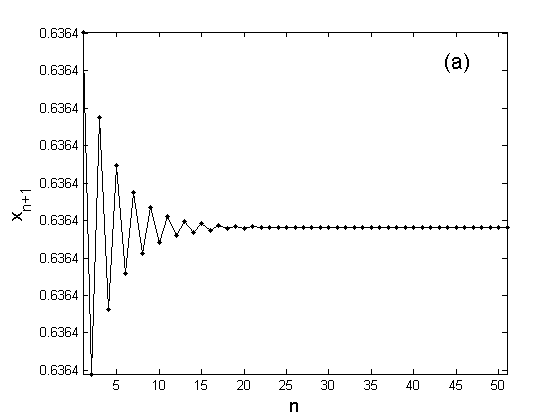
\includegraphics{Figuras/logistico1.png}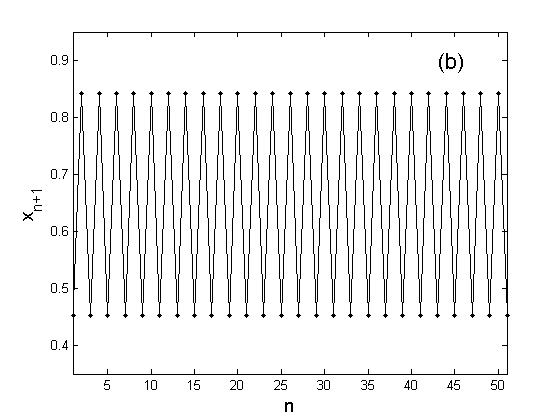
\includegraphics{Figuras/logistico2.png}}\\ \resizebox{15cm}{!}{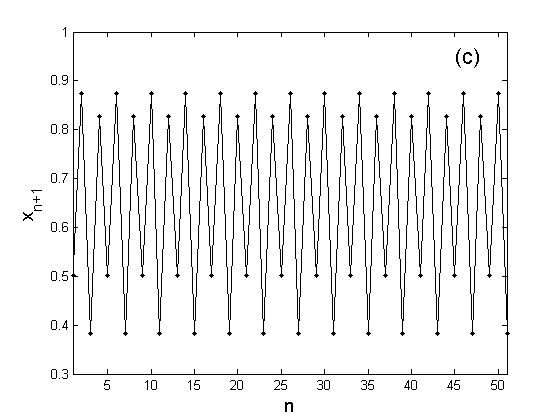
\includegraphics{Figuras/logistico3.png} 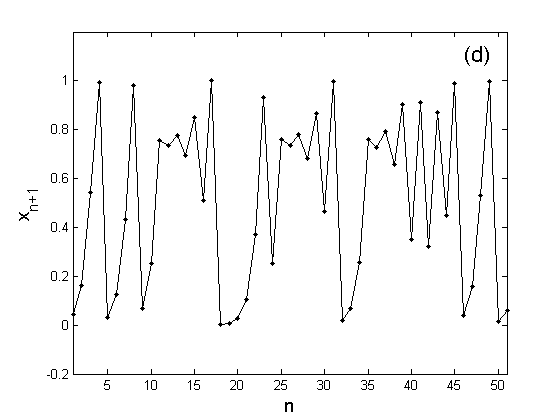
\includegraphics{Figuras/logistico4.png}}
%\caption{Séries temporais obtidas a partir da iteração do mapa~(\ref{equalogis1}) com condição inicial fixa $x_{0}=0.01$ e para valores de $\lambda$ dados, respectivamente por $2.75$, $3.4$, $3.5$ e $4.0$.}
%\label{figuralogis}
%\end{figure}
%
%O mapa logístico também evidencia outra característica dos sistemas caóticos: a \textit{imprevisibilidade}, ou seja, o conhecimento do valor aproximado do estado do sistema não permite predizer, de maneira imediata, sua evolução posterior para qualquer tempo futuro. Este comportamento está associado à \textit{sensibilidade às variações nas condições iniciais} e ao fato de não se conseguir obter com precisão infinita o valor real do estado. Para o Sistema~(\ref{equalogis1}) valores muito próximos de uma condição inicial $x_0$ conduzem, após algumas poucas iterações, a órbitas completamente distintas, conforme pode ser observado na Figura~\ref{figuralogis2}.
%
%\begin{figure}[ht]
%\centering
%\resizebox{15cm}{!}{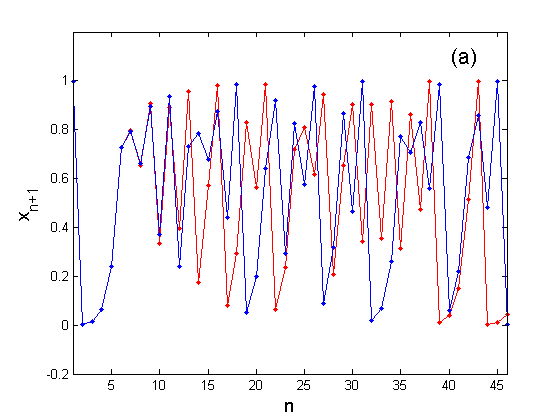
\includegraphics{Figuras/logisticoci.png}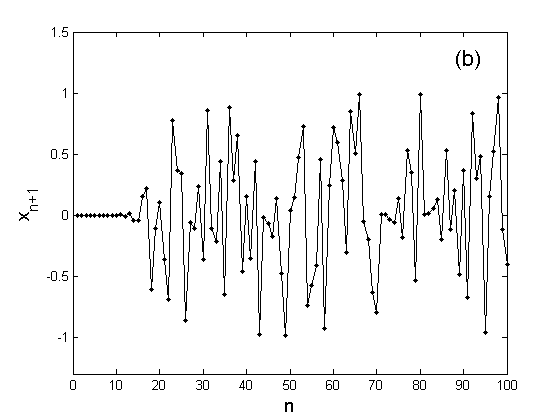
\includegraphics{Figuras/logisticocidiff.png}}
%\caption{(a) Séries temporais obtidas pela iteração do mapa~(\ref{equalogis1}) para valores muito próximos de $x_0$. A curva em azul corresponde à órbita gerada com condição inicial $x_{0}=0.01$, enquanto que a curva em vermelho corresponde à órbita gerada com condição inicial $x_{0}=0.010001$. (b) as diferenças associadas às duas órbitas.}
%\label{figuralogis2}
%\end{figure}
%
%As trajetórias ou órbitas de um sistema caótico oscilam confinados em uma região limitada do espaço de estados, sem entretanto, apresentar periodicidade~\cite{alligood/97}. No interior desta região, as variáveis de estado exibem valores correspondentes a pontos no espaço de fase para os quais as trajetórias caóticas, iniciando em um número significativo de condições iniciais, passam arbitrariamente próximas, infinitas vezes, à medida que o sistema evolui no tempo. Isto é, uma vez iniciada a evolução do sistema, sua trajetória é \textit{atraída} para um sub-conjunto de pontos do espaço de fase, conhecido como \textit{atrator caótico}, e ali permanece percorrendo este sub-conjunto indefinidamente. O conjunto de todas as condições iniciais que converge para o atrator caótico é chamado \textit{bacia de atração} do atrator~\cite{alligood/97}.
%
%Se a estrutura geométrica criada por estados assintóticos das trajetórias for um fractal, este é denominado atrator estranho. Atratores caóticos apenas ocorrem em sistemas dissipativos. Sobre este atrator, a dinâmica é caracterizada por \textit{esticamentos} e \textit{dobras}; o primeiro fenômeno é responsável pela divergência de trajetórias próximas e o último é responsável pela contração da dinâmica para uma região finita em um subespaço de dimensão $\leq m$.  Em contraste com sistemas não-caóticos que possuem atratores de dimensão inteira como pontos atrativos (que geram soluções estacionárias) e ciclos limites (que produzem soluções periódicas), sistemas caóticos podem estar associados a atratores caóticos caracterizados por uma dimensão não-inteira $d$. Esta dimensão é uma propriedade do atrator, independentemente de uma trajetória em particular.
%
%Segundo \citeonline{ruelle/91} atratores caóticos que apresentam o fenômeno da \textit{sensibilidade às variações nas condições iniciais}, correspondem à excitação de um número finito de graus de liberdade e embora tais atratores possuam dimensão finita, a análise em termos de freqüências temporais revela um \textit{espectro contínuo de freqüências}. 
%
%O mapa de Hénon é um exemplo de sistema dinâmico discreto, que apresenta um atrator caótico em sua dinâmica. Este mapa é descrito pelas equações 
%\begin{equation}
%\begin{array}{lcl} x_{n+1} & = & 1-ax_{n}^2+y_{n} \\ 
%                   y_{n+1} & = & bx_{n} \\
%\end{array}
%\label{eqhenon}
%\end{equation}
%sendo $a$ e $b$ parâmetros do mapa. Para valores de $a=1.4$ e $b=0.3$, este sistema apresenta um comportamento irregular e aperiódico que se desenvolve em um atrator caótico e estranho. O atrator de Hénon e uma seqüência de sua ampliação são mostrados na Figura~\ref{figurahenonsimilar}. A dimensão fractal~\cite{mandelbrot/82} associada a esse atrator é de $1.265$, sendo evidente seu caráter auto-similar - característica típica de atratores estranhos~\cite{alligood/97}.
%
%\begin{figure}[ht]
%\centering
%\resizebox{15cm}{!}{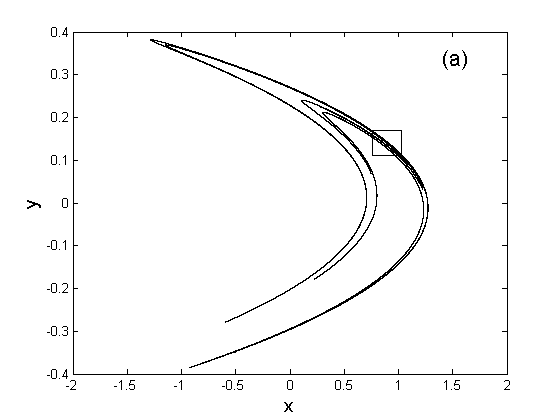
\includegraphics{Figuras/henon.png}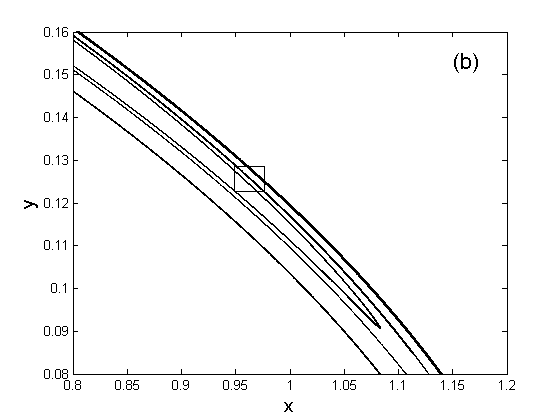
\includegraphics{Figuras/henonamp1.png}}\\ \resizebox{15cm}{!}{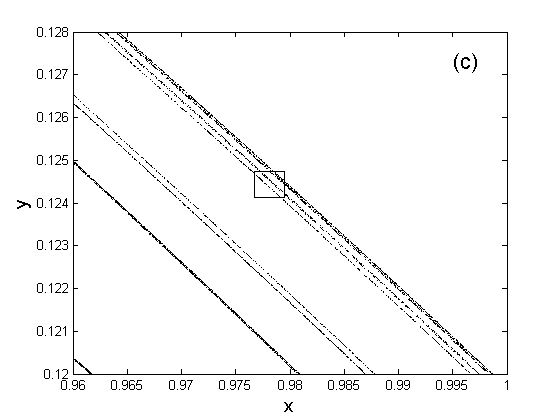
\includegraphics{Figuras/henonamp2.png} 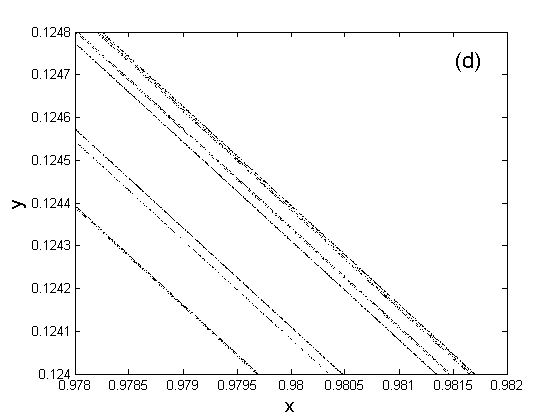
\includegraphics{Figuras/henonamp3.png}}
%\caption{Autosimilaridade do atrator de Hénon. Os pequenos quadrados indicam as regiões de ampliação. (a) $10^3$ iterações. (b) $10^5$ iterações. (c) $10^6$ iterações. (d) $10^7$ iterações.}
%\label{figurahenonsimilar}
%\end{figure}
%
%Para medir a taxa de divergência de trajetórias e, portanto, quantificar a sensibilidade às variações nas condições iniciais, utilizam-se os \textit{expoentes característicos de Lyapunov}. Essa caracterização constitui um dos principais critérios para definir comportamento caótico em sistemas dinâmicos.  
%
%Os expoentes de Lyapunov contêm informações sobre a taxa média com que as trajetórias exponencialmente divergem ou convergem dentro do atrator. Eles estão relacionados às direções de expansão ou contração no espaço de fase~\cite{wolf/85}. Um sistema caótico é caracterizado por uma divergência exponencial de condições iniciais próximas, o que implica em pelo menos um expoente de Lyapunov estritamente positivo. A magnitude do maior expoente positivo (caso exista) reflete a escala temporal sobre a qual o sistema dinâmico torna-se imprevisível~\cite{jaramillo/93}. 
%
%A estimativa dos expoentes de Lyapunov de um sistema dinâmico dissipativo $m$-dimensional requer que se acompanhe a evolução de uma esfera infinitesimal $m$-dimensional de condições iniciais. Com o passar do tempo, a esfera evolui para a forma de um elipsóide. Os expoentes de Lyapunov são definidos tomando o eixo principal do elipsóide. Especificamente, o $i$-ésimo maior expoente $\lambda_{i}$ é definido em termos da taxa de crescimento do $i$-ésimo maior eixo principal, $P_{i}$:
%\begin{equation}
%\lambda_{i}=\lim_{t\rightarrow\ \infty}\frac{1}{t}\log_{2}\left[\frac{P_{i}(t)}{P_{i}(0)}\right]
%\label{eqlyapheuristico}
%\end{equation}
% 
% O conceito de expoente de Lyapunov pode ser apresentado, de forma heurística, considerando uma bola infinitesimal de dimensão $m$ em um espaço de estado. Durante a evolução desse sistema a bola se torna um elipsóide, porém ainda infinitesimal. Denotando o eixo principal deste elipsóide por $\epsilon_{i}(t)\:(i=1,2,\ldots,m)$, os expoentes de Lyapunov $\lambda_{i}$ são determinados por
%  
% \begin{equation}
% \epsilon_{i}(t)\approx\epsilon_{i}(0)e^{\lambda_{i}t}
% \label{eqlyapheuristico}
% \end{equation}
% 
%A soma dos expoentes $\lambda_{i}$, que descrevem a contração do volume, deve ser negativa já que o sistema dinâmico é dissipativo. Desta forma, se um atrator caótico é resultante de esticamentos e dobras, isto requer que pelo menos um dos $\lambda_{i}$ seja positivo. Inversamente, um expoente de Lyapunov positivo implica sensibilidade às variações nas condições iniciais, e desta forma comportamento caótico~\cite{grassbergerstratt/83}.
%
%A Figura~\ref{fighenonlyapunov} apresenta a evolução ao longo do tempo dos expoentes de Lyapunov associados ao Sistema~(\ref{eqhenon}) com condição inicial $(x_{0},y_{0})=(1,1)$. Pode-se observar que um destes expoentes é positivo e dado por $\lambda_{1}=0.42$. Aproximações para os expoentes de Lyapunov, com condições iniciais diferentes, tendem para o mesmo valor $\lambda_{1}$, já que o Sistema~(\ref{eqhenon}) é ergódico. Esse comportamento parece indicar que o sistema apresenta dinâmica caótica.
%
%\begin{figure}[ht]
%\centering \resizebox{10cm}{!}{\includegraphics{Figuras/henonlyapunov.png}} 
%\centering \resizebox{13cm}{!}{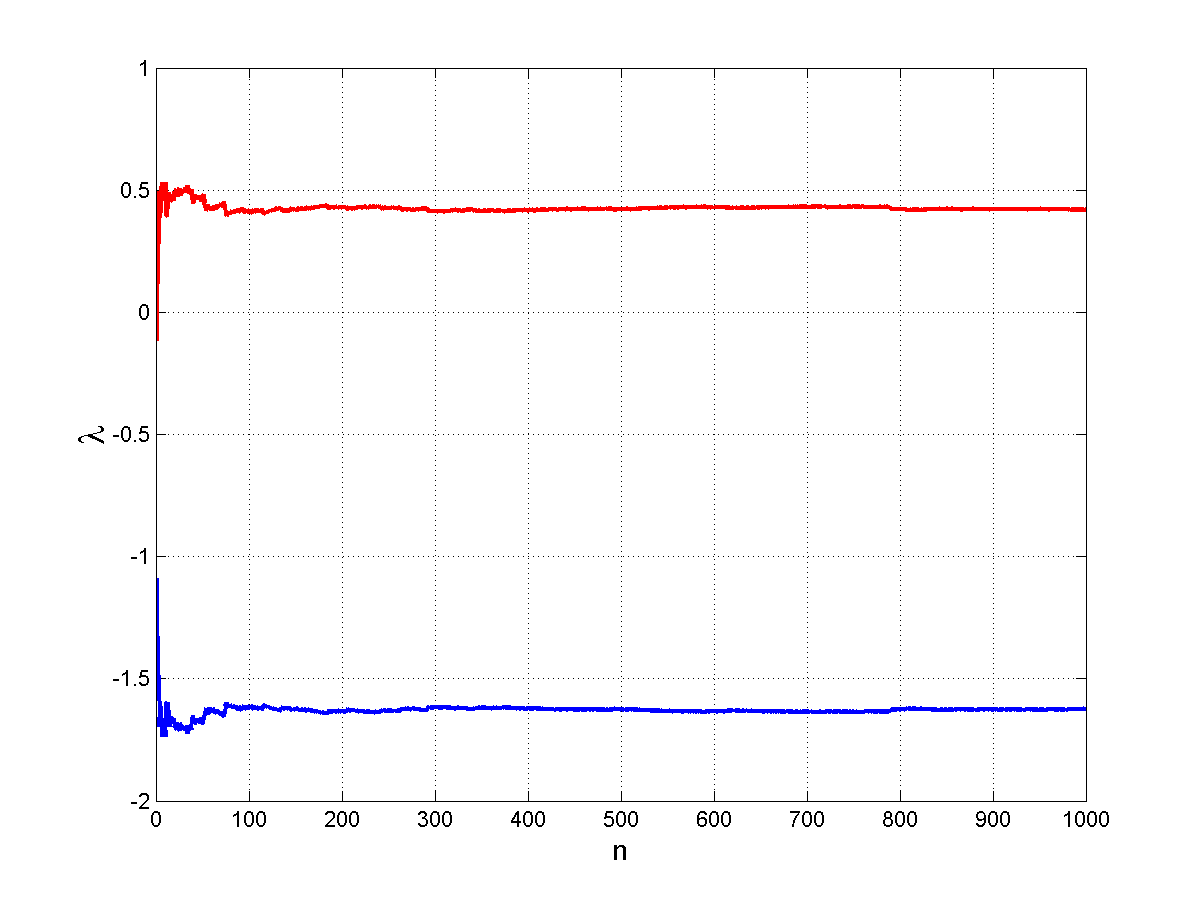
\includegraphics{Figuras/henonlyapunovgrid.png}} 
%\caption{Expoentes de Lyapunov associados ao mapa de Hénon (\ref{eqhenon}) com $a=1.4$ e $b=0.3$.}
%\label{fighenonlyapunov}
%\end{figure}
%
%O artigo clássico de \citeonline{lor/63} foi um dos primeiros trabalhos a descrever movimentos caóticos a partir de um sistema de EDO's, como uma aproximação para a dinâmica de uma camada de fluido convectiva. Suponha que esta camada seja mais quente na base do que no topo (conforme a Figura~\ref{figconveclorenz}), e que a diferença de temperatura $\Delta t$ seja suficiente grande. Sob estas condições o ar mais quente se eleva, deslocando o ar mais frio que está por cima, provocando um movimento convectivo permanente. Se a diferença de temperatura aumentar ainda mais, o escoamento convectivo permanente é perturbado e se instala um movimento turbulento mais complicado~\cite{boyce/99}.
%
%\begin{figure}[ht]
%\centering \resizebox{13cm}{!}{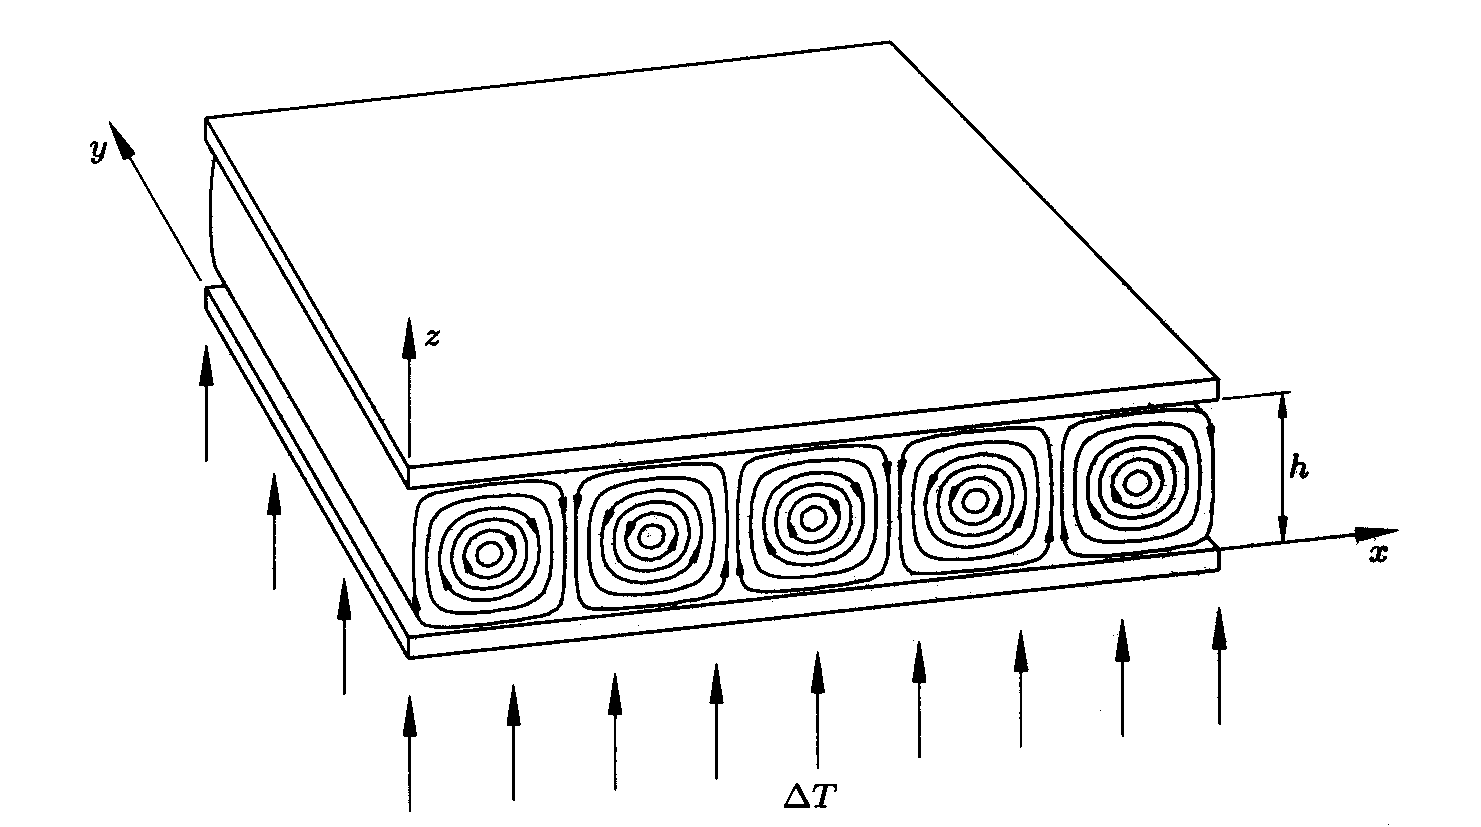
\includegraphics{Figuras/rolo.png}} 
%\caption{Movimento convectivo de uma camada de fluido, com diferença de temperatura $\Delta t$ entre a placa inferior e a superior que o delimita.}
%\FONTE{Adaptada de \citeonline{argyris/94}.}
%\label{figconveclorenz}
%\end{figure}
%
%Ao investigar este fenômeno, Lorenz foi levado, por um processo complexo cuja descrição não é o enfoque deste trabalho, ao sistema autônomo não-linear de EDO's
%\begin{equation}
%\begin{array}{ccc} dx/dt & = & \sigma(-x+y) \\ dy/dt & = & rx-y-xz \\ dz/dt & = & -bz+xy \end{array}
%\label{eqsistemalorenz}
%\end{equation}
%
%As Equações~(\ref{eqsistemalorenz}) são comumente denominadas equações de Lorenz. Pode-se observar que a segunda e a terceira equações envolvem não-linearidades quadráticas. A variável $x$, está relacionada à intensidade do movimento do fluido, enquanto as variáveis $y$ e $z$ estão relacionadas a variações de temperatura nas direções horizontal e vertical. As equações de Lorenz também envolvem três parâmetros $\sigma$, $r$ e $b$, todos reais e positivos. Os parâmetros $\sigma$ e $b$ dependem do material e das propriedades geométricas da camada fluida. No caso da atmosfera, valores razoáveis destes parâmetros são 
%$\sigma=10$ e $b=8/3$~\cite{lor/63}. O parâmetro $r$, por outro lado, é proporcional à diferença de temperatura $\Delta t$, e em todas as simulações posteriores assumirá valor $28$. Desta forma, o Sistema~(\ref{eqsistemalorenz}) assume uma forma particular, dada por
%\begin{equation}
%\begin{array}{ccc} dx/dt & = & 10(-x+y) \\ dy/dt & = & 28x-y-xz \\ dz/dt & = & -8/3z+xy \end{array}
%\label{eqsistemalorenzpart}
%\end{equation}
%
%A Figura~\ref{figlorenzx}(a) apresenta um gráfico de valores calculados de $x$ em função de $t$, ou seja, a evolução no tempo da variável de estado $x$, que é parte da solução do Sistema~(\ref{eqsistemalorenzpart}). Note que a solução oscila entre valores positivos e negativos de uma maneira aparentemente errática. Na realidade, o gráfico de $x$ contra $t$ assemelha-se ao de uma oscilação aleatória, embora as equações de Lorenz sejam inteiramente determinísticas e a solução seja completamente determinada pelas condições iniciais. Não obstante, a solução aparenta, também, uma certa \textit{regularidade}, pois a freqüência e a amplitude das oscilações são essencialmente constantes no tempo.
%
%As soluções das equações de Lorenz são também muito sensíveis a perturbações nas condições iniciais. A Figura~\ref{figlorenzx}(b) mostra os gráficos dos valores calculados de $x$ contra $t$ para duas soluções com condições iniciais bastante próximas. As duas soluções ficam bastante próximas uma da outra, até $t$ nas vizinhanças de $10$, e depois se tornam bastante diferentes, parecendo não ter qualquer relação mútua. Esta propriedade atraiu particularmente a atenção de Lorenz no seu trabalho original sobre as equações, e que tal fato deve estar relacionado à impossibilidade de se ter previsões a longo prazo das condições meteorológicas~\cite{boyce/99}.
%
%\begin{figure}[ht]
%\centering 
%\resizebox{15cm}{!}{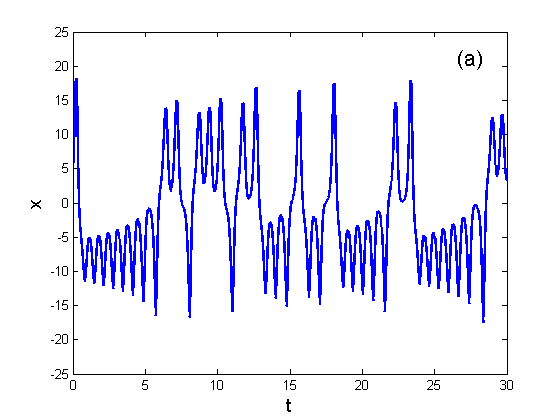
\includegraphics{Figuras/lorenzst.png}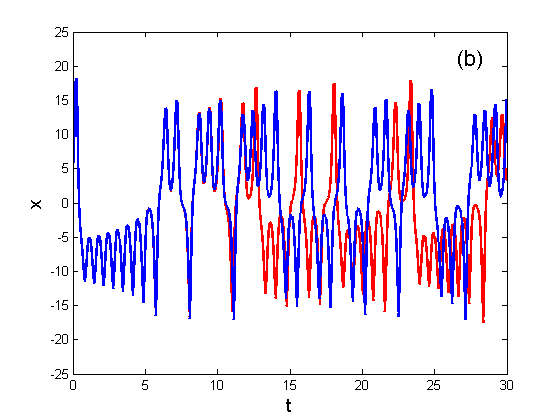
\includegraphics{Figuras/lorenzstci.png}}
%\caption{Séries temporais obtidas a partir da integração do Sistema~(\ref{eqsistemalorenzpart}). (a) condição inicial de $(5,5,5)$. (b) condição inicial da curva em azul é de $(5,5,5)$ enquanto que a da curva em vermelho é de $(5.01,5,5)$.}
%\label{figlorenzx}
%\end{figure}
%
%A Figura~\ref{figlorenzatratorproj} apresenta uma trajetória que principia em $(5,5,5)$ no espaço de fase tridimensional, que se desenvolve em um atrator caótico cuja dimensão de capacidade é de aproximadamente $2.16$~\cite{argyris/94}, como também suas projeções nos planos $xy$, $xz$ e $yz$. Pode-se observar que a trajetória sobre o atrator nunca repete o mesmo caminho; contudo, ela está confinada (atraída) em uma região limitada do espaço de fase. Tal trajetória se alterna sobre um dos dois lóbulos, onde cada um deles contém um ponto crítico instável, e este processo é repetido indefinidamente.
%
%\begin{figure}[ht]
%\centering \resizebox{13cm}{!}{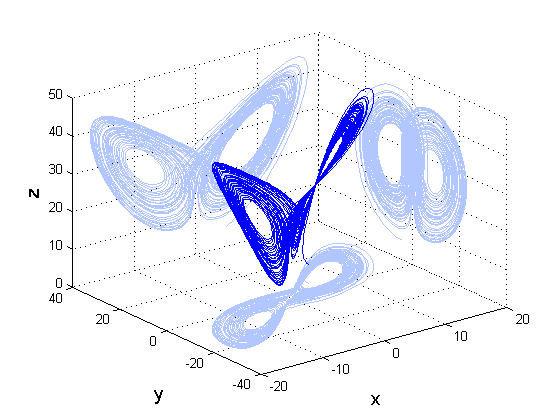
\includegraphics{Figuras/lorenzatratorproj.png} } 
%\caption{O atrator caótico de Lorenz com condição inicial $(5,5,5)$, e suas projeções nos planos $xy$ e $xz$ e $yz$.}
%\label{figlorenzatratorproj}
%\end{figure}
%
%Segundo \citeonline{wolf/85} os expoentes de Lyapunov associados ao Sistema~(\ref{eqsistemalorenz}) (com $\sigma=16$ e $b=4.0$ e $r=45.92$) são dados por
%$\lambda_{1}=2.16$, $\lambda_{2}=0$ e $\lambda_{3}=-32.4$. Desta forma, a dinâmica caótica presente nesse sistema parece se confirmar pela presença de um expoente de Lyapunov positivo~\cite{wolf/85}.
%
%Quando as equações que governam um sistema dinâmico são conhecidas, o estudo das características de suas soluções e de seus invariantes podem revelar comportamentos complexos e interessantes. Porém, em situações reais raramente se dispõe de um conjunto de equações diferenciais ou mesmo um mapa que descreva o comportamento do sistema. Em geral, monitora-se uma única variável, a partir de um experimento que se sabe de antemão depender de outras variáveis. Desta forma, obtém-se uma série temporal de medidas semelhantes às exibidas pelas Figuras~(\ref{figlorenzx}) ou (\ref{figuralogis}) (admitindo-se o não-conhecimento de suas equações) e não se tem acesso às outras variáveis relevantes. A análise de séries temporais com base na teoria de sistemas dinâmicos é um dos temas centrais do Capítulo~\ref{caputiltecnicas}.
%
% 
%\section{Turbulência}
%\label{secturb}
%
%\subsection{Introdução}
%
%O primeiro esboço de um fluxo turbulento, com diversos graus de realismo, foi feito por Leonardo da Vinci no século XV (conforme Figura~\ref{figleonardo}). Para ele o movimento da água em ``redemoinhos'' era devido em parte à sua corrente principal, como também por movimentos contrários e aleatórios. Da Vinci nomeou tal fenômeno de ``la turbolenza''~\cite{richter/70}. 
%
%\begin{figure}[ht]
%\centering \resizebox{13cm}{!}{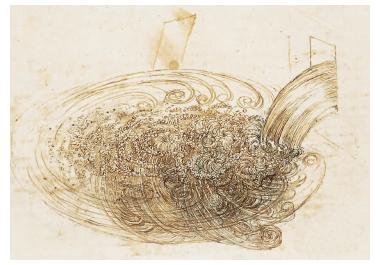
\includegraphics{Figuras/DaVinci3.png}}
%\centering \resizebox{10cm}{!}{\includegraphics{Figuras/DaVincipb.png}} opcao preto e branco!!!
%\caption{Ilustração de Leonardo da Vinci de um fluxo em redemoinhos.}
%\FONTE{\citeonline{ecke/05}}
%\label{figleonardo}
%\end{figure}
%
%Dois aspectos das observações de Leonardo da Vinci têm permanecido até os dias de hoje. Primeiro, a separação do fluxo em uma parte média e outra flutuante, que antecipou em quase $400$ anos a aproximação feita por Osborne Reynolds. Segundo, a identificação de ``vórtices'' como elementos intrínsecos no movimento turbulento. O termo ``vórtice'', usado aqui, refere-se a vários tipos de estruturas turbulentas presentes no escoamento, associadas, por exemplo, ao campo de velocidade de um fluido~\cite{ecke/05}.
%
%\subsection{As equações de Navier Stokes}
%
%Após as descrições feitas por Leonardo da Vinci, o maior avanço na análise do movimento de um fluido foi por meio de equações dinâmicas, como as equações de Navier Stokes (escritas durante o século XIX), que descrevem a taxa de variação da quantidade de movimento em cada ponto de um fluido viscoso. Para um fluido com densidade constante $\rho$ e viscosidade cinemática constante $\nu$, as equações de Navier-Stokes assumem a forma 
%
%\begin{equation}
%\frac{\partial u}{\partial t}+u\cdot\bigtriangledown u=-\frac{\bigtriangledown P}{\rho}+\nu\bigtriangledown ^2u
%\label{eqns1}
%\end{equation}
%
%\begin{equation}
%\bigtriangledown\cdot u=0
%\label{eqns2}
%\end{equation}
%
%Essas equações modelam o escoamento de fluidos incompressíveis, laminares e turbulentos, a partir de condições convenientes impostas nos contornos do fluido. A Equação~(\ref{eqns2}) é a condição de continuidade (sem fontes nem sumidouros), a variável $u(x,t)$ é o campo de velocidade do fluido (incompressível), e $P(x,t)$ é o campo de pressão determinado pela preservação da incompressibilidade~\cite{ecke/05}. O termo $\nu\bigtriangledown ^2u$ representa a contribuição das forças dissipativas lineares da Equação~(\ref{eqns1}), enquanto o termo $u\cdot\bigtriangledown u$ representa a contribuição das forças de inércia não lineares da mesma equação.
%
%A Figura~(\ref{figvulcao}) apresenta a erupção explosiva do Monte St. Helens em sucessivas ampliações, mostrando estruturas em diversos comprimentos de escala. A grande diferença de velocidade, resultante de forças de cisalhamento aplicadas produzem um fluido fortemente turbulento, um estado que pode ser definido como uma solução das equações de Navier-Stokes cujas características exibem flutuações espacial e temporal~\cite{ecke/05}.
% 
%A Equação~(\ref{eqns1}) (quando multiplicada por $\rho$ fornece força por unidade de volume) é simplesmente a lei de Newton para um fluido: força é igual massa vezes aceleração. O lado esquerdo da mesma é a aceleração do fluido\footnote{A aceleração de um fluido é, por definição, a derivada segunda (no tempo) da trajetória do fluido lagrangiano $x(t)$, que descreve o movimento do fluido que estava inicialmente na posição $x(0)$. A primeira derivada é a velocidade lagrangiana do fluido, $dx(t)/dt$ que está relacionada com a velocidade euleriana do fluido por $dx(t)/dt=u(t,x(t))$. Devido $u$ ser uma função do tempo $t$ e da posição $x(t)$, que é por si mesma função do tempo, a expressão euleriana para a derivada segunda lagrangiana (a aceleração do fluido) é obtida através da regra da cadeia e igual a $du/dt=\partial u/\partial t +u\cdot\bigtriangledown u$.}, e seu lado direito é a soma das forças por unidade de massa sobre uma unidade de volume do fluido.
%
%Acredita-se que as equações de Navier-Stokes contêm toda a informação sobre o escoamento turbulento. Embora o problema físico possa em princípio ser completamente revelado pela solução dessas equações, dadas as condições iniciais e de contorno, há uma grande dificuldade devido à sua natureza não-linear~\cite{welter/06}. Mesmo que fosse possível obter uma solução completa de um escoamento turbulento, onde o campo de velocidades $u(x,t)$ pudesse ser conhecido com exatidão em cada ponto do espaço e a cada instante de tempo, esse tipo de conhecimento seria inaplicável devido à dificuldade de armazenagem e processamento da enorme quantidade de informação. Assim, devido os graus de liberdade envolvidos em um escoamento turbulento serem muito grandes,\footnote{Segundo \citeonline{lulandlif/59}, o número de graus de liberdade em um escoamento turbulento é proporcional a $R_{e}^{9/4}$, onde $R_{e}$ é denominado número de Reynolds.} uma das abordagens mais utilizadas é o tratamento estatístico das quantidades de interesse.
%
%\begin{figure}[ht]
%\centering \resizebox{15cm}{!}{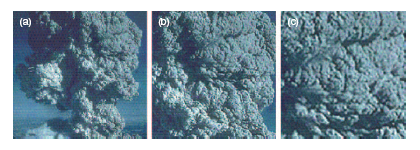
\includegraphics{Figuras/vulcaoturb.png}}
%\caption{(a) A estrutura turbulenta de uma erupção vulcânica do Monte St. Helens, (b) ampliação por um fator de $2$, (c) ampliação por outro fator de $2$. 
%A escala característica da coluna de fumaça é de aproximadamente $5$ Km. }
%\FONTE{\citeonline{ecke/05}}
%\label{figvulcao}
%\end{figure}
%
%
%\subsection {O Número de Reynolds}
%
%Como se sabe, é possível distinguir entre dois tipos de escoamentos. Os escoamentos laminares, que são suaves e determinísticos, e os escoamentos turbulentos, que são abruptos e irregulares no tempo e no espaço. A transição do escoamento laminar para o escoamento turbulento é considerado um dos problemas mais complexos em mecânica dos fluidos. As teorias de transição do escoamento laminar para o turbulento são baseadas nas pequenas perturbações no escoamento. Estas perturbações teriam sua origem nas colisões intermoleculares, e dependendo da estabilidade do escoamento, seriam amplificadas ao passar do tempo e então o escoamento torna-se turbulento~\cite{welter/06}.
%
%Na tentativa de criterizar a transição para a turbulência, \citeonline{reinolds/1895} definiu uma relação entre forças inerciais e viscosas que atuam nos fluidos. Esta razão, um parâmetro adimensional, seria o ponto crítico de transição entre escoamentos laminares e turbulentos. Hoje chamado de \textit{número de Reynolds} ($R_{e}$), este parâmetro é proporcional à razão entre a contribuição das forças inerciais não lineares da Equação~(\ref{eqns1}) e à contribuição das suas forças dissipativas lineares.
%
%Se $U$ é uma velocidade característica do escoamento e $L$ é uma escala de comprimento característico, então as forças inerciais são da ordem de $U^{2}/L$ e as forças viscosas são da ordem de $\nu U/L^{2}$. Assim, o número de Reynolds do escoamento pode ser caracterizado por
%
%\begin{equation}
%R_{e}=\frac{LU}{\nu}
%\label{eqreynolds2}
%\end{equation}
%\newline
%
%Quando o numerador é muito maior que o denominador em~(\ref{eqreynolds2}), o valor de $R_{e}$ é grande e desta forma o fluxo é turbulento, caso contrário o fluxo é laminar (admitindo-se L constante). Em geral, considera-se que o número de Reynolds crítico está entre $2300$ e $3000$. Para números de Reynolds menores que o número de Reynolds crítico, a não-linearidade presente nas equações de Navier Stokes pode ser omitida, e as soluções analíticas para tais equações correspondem a fluxos laminares. Para número de Reynolds maiores que o número de Reynolds crítico não há soluções estacionárias estáveis e o fluido torna-se turbulento. Em particular, o fluxo se encontra na turbulência completamente desenvolvida quando $R_{e}$ é muito maior que aquele obtido na transição para a turbulência, levando-se em conta um conjunto particular de forças e condições de contorno. Na natureza e em laboratórios os escoamentos são em sua maioria turbulentos. Em experimentos laboratoriais em túnel de vento $R_{e}\sim 10^{5}$ e na camada limite atmosférica $R_{e}\sim 10^{7}$~\cite{welter/06}. 
%
%O efeito da variação do número de Reynolds $R_{e}$ em um fluido pode ser vista claramente na Figura~\ref{reynolds1}, que mostra graficamente o padrão de um fluxo uniforme em um cilindro circular. O fluxo, neste caso, é visualizado por uma fumaça ejetada da superfície do cilindro.
%
%Para o estágio (a), $R_{e}\leq 1$, o fluxo é estacionário e não se separa do cilindro. Em (b), $1<R_{e}<10$, o fluxo é ainda estacionário mas um par de vórtices aparecem atrás do cilindro, que aumenta com o incremento de $R_{e}$. Em (c), $10<R_{e}<10^2$, os vórtices estão separados alternativamente do cilindro e alinhados em duas fileiras de vórtices, o conhecido fenômeno dos vórtices de Kármán~\cite{tomomasa/2000}. Neste caso, o fluxo não é mais estacionário e passa a ser periódico.
%
%Em (d), $10^2<R_{e}<10^5$, as fileiras de vórtices tornam-se irregulares e surge um fluxo turbulento, porém ainda laminar fora dele. Em (e), $R_{e}>10^5$, a região torna-se composta de uma grande variedade de vórtices em tamanho e direção, ou seja, o estágio da turbulência completamente desenvolvida. Acima de um certo valor crítico de $R_{e}$, no intervalo $10^5<R_{e}<10^6$, o fluxo no contorno do cilindro também torna-se turbulento.
%
%\begin{figure}[ht]
%\centering \resizebox{9cm}{!}{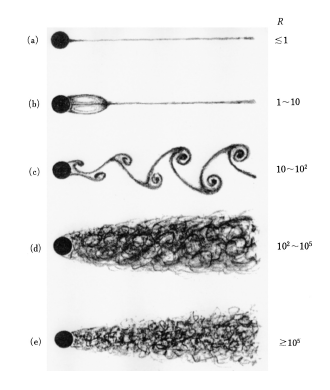
\includegraphics{Figuras/reynoldstomomasa.png}}
%\caption{Mudança no padrão do fluxo de acordo com o número de Reynolds $R_{e}$.}
%\FONTE{\citeonline{tomomasa/2000}}
%\label{reynolds1}
%\end{figure}
%
% As várias simetrias permitidas pela equação de Navier-Stokes são sucessivamente quebradas com o incremento de $R_{e}$, ou seja, quando o fluxo deixa de ser laminar e passa a ser turbulento. Porém, em número de Reynolds ainda mais elevados há uma tendência das simetrias perdidas serem restauradas no senso estatístico, este é o caso da turbulência plenamente desenvolvida, mencionada anteriormente. 
%
%\subsection{Caracterização clássica da turbulência}
%
%\citeonline{lumpano/64} apontam algumas propriedades de um campo turbulento, a saber
%\begin{itemize}
%\item Turbulência é rotacional e dissipativa, isto é, energia mecânica é transformada em calor;
%\item Turbulência é tridimensional; 
%\item Turbulência é não-linear. Todas as escalas estão acopladas entre si no tempo e no espaço;
%\item Turbulência é estocástica. Na prática não importa com qual cuidado as condições de um experimento sejam reproduzidas, o campo de velocidades não poderá ser predito em detalhes; 
%\item Turbulência é um fenômeno contínuo;
%\item Turbulência é difusiva. Um ponto marcado em um fluido turbulento irá vaguear, excursionando para longe de sua posição inicial. Este comportamento é responsável pelo transporte de quantidades (massa, momentum e calor).
%\end{itemize}
%
%O caráter estocástico da turbulência foi questionado por \citeonline{ruelltak/71}. Tais autores introduziram uma interpretação alternativa dos processos turbulentos com base na teoria de sistemas dinâmicos, mais especificamente via ``atratores caóticos de baixa dimensão''. Este assunto será tratado em detalhes na Seção~(\ref{seccaosurb}).
%
%A Figura~\ref{figvelocidadevert} apresenta a evolução de uma variável turbulenta ao longo do tempo, amostrada à $60$Hz. Pode-se observar, que mesmo à uma taxa de amostragem alta, não é possível observar uma variação suave de tal variável com o tempo. O mesmo comportamento é esperado com respeito ao espaço.
%
%\begin{figure}[ht]
%\centering \resizebox{13cm}{!}{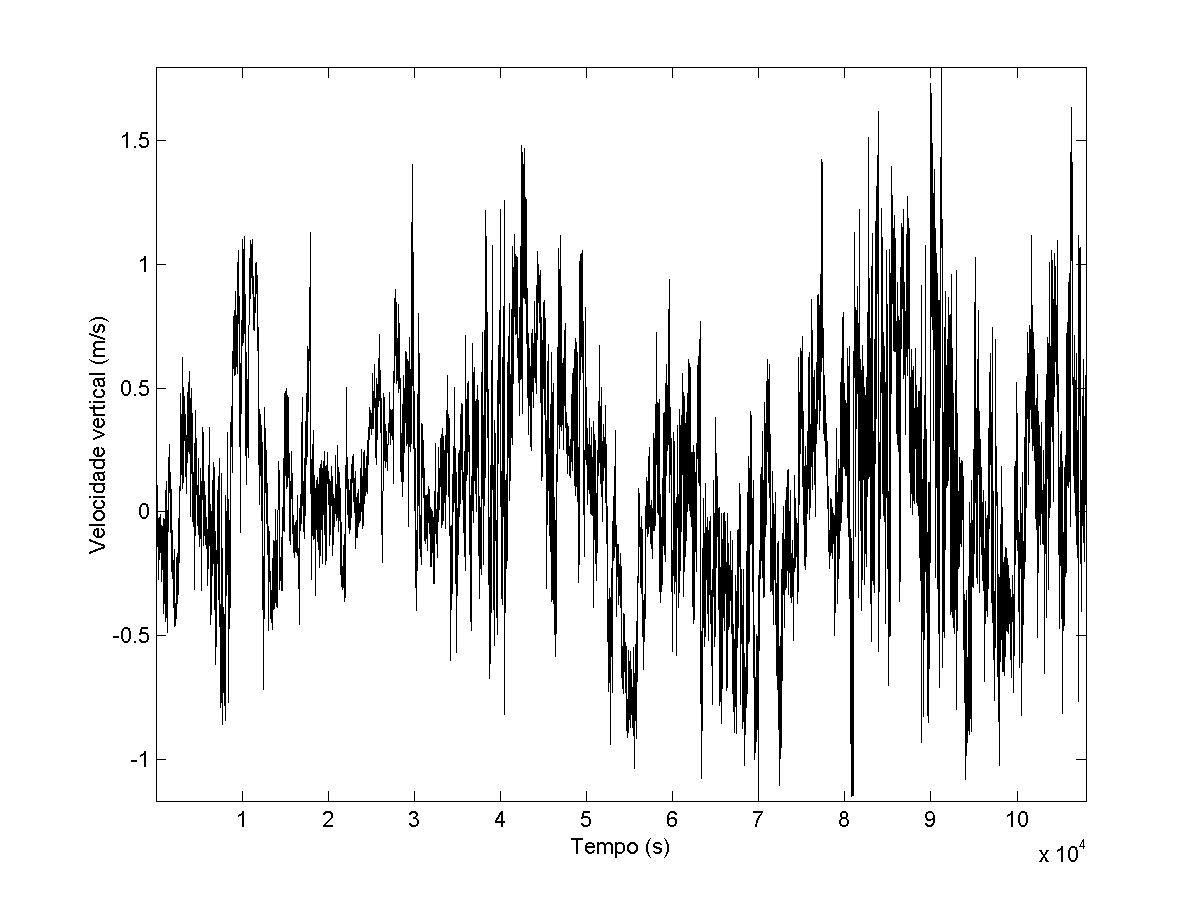
\includegraphics{Figuras/velocidadevert.png}}
%\caption{Evolução temporal de uma variável turbulenta amostrada à $60$Hz.}
%\label{figvelocidadevert}
%\end{figure}
%
%Pode-se imaginar, entretanto, que uma variável turbulenta, como a da Figura~\ref{figvelocidadevert}, é uma composição de um número muito grande de harmônicos e, desta forma, pode-se pensar que a turbulência é composta de uma superposição de vários harmônicos acoplados entre si não linearmente. Estes harmônicos podem ser denominados vórtices. Seguindo esta idéia, um campo turbulento é composto de uma superposição de um número muito grande de vórtices com vários números de onda. Naturalmente, surge a necessidade de se conhecer a distribuição da energia cinética entre estes números de onda~\cite{welter/06}. 
%
%Segundo \citeonline{arya/88}, em escoamentos com elevado número de Reynolds a \textit{Energia Cinética Turbulenta} (ECT) é fornecida aos vórtices nas maiores escalas turbulentas (da ordem de $10^3$m) e, então, dissipada pelos vórtices nas menores escalas (da ordem de $10^{-3}$). A transferência dessa energia ocorre, possivelmente, por meio de um processo de cascata envolvendo todas as escalas intermediárias. Essa idéia foi proposta por Richardson em $1922$~\cite{monin/71} e foi desenvolvida por Kolmogorov em sua teoria sobre turbulência desenvolvida (teoria K41) e, ainda hoje, é objeto de muita discussão~\cite{frisch/96,nelkin/92}. Vórtices maiores colapsam-se em vórtices menores, sucessivamente, até atingirem as menores escalas, onde são destruídos pelas forças viscosas. Desta forma, os vórtices menores não estão diretamente ligados aos processos geradores de energia cinética turbulenta nas maiores escalas (flutuabilidade térmica e cisalhamento vertical da velocidade do vento), permitindo que as escalas intermediárias dessa cascata de energia tenham atributos universais a todos os escoamentos turbulentos. 
%
%A Figura~\ref{espectroesboco} é uma representação esquemática do espectro da ECT. A região $1$ é a de produção de ECT, onde o escoamento médio fornece energia aos maiores vórtices turbulentos através da flutuabilidade e do cisalhamento do vento. Kolmogorov, em $1941$, propôs a \textit{Teoria do Equilíbrio Universal} sobre a similaridade e isotropia da turbulência desenvolvida na pequena escala~\cite{monin/71}. De acordo com essa teoria, para escoamentos com número de Reynolds suficientemente elevados, na Região $2$ da Figura~\ref{espectroesboco}, denominada de \textit{Subdomínio Inercial} (SI), a turbulência é homogênea e isotrópica e nela as propriedades médias do escoamento dependem diretamente apenas de $\epsilon$, a \textit{taxa de dissipação de ECT por unidade de massa}. Ainda, de acordo com a Teoria do Equilíbrio Universal, a região $3$ é onde a ECT transferida pela região $2$ é convertida em calor pela ação da viscosidade, fazendo com que outro parâmetro além de $\epsilon$ seja importante nessa região - a \textit{viscosidade cinemática} $\nu$.
%
%
%\begin{figure}[ht]
%\centering \resizebox{13cm}{!}{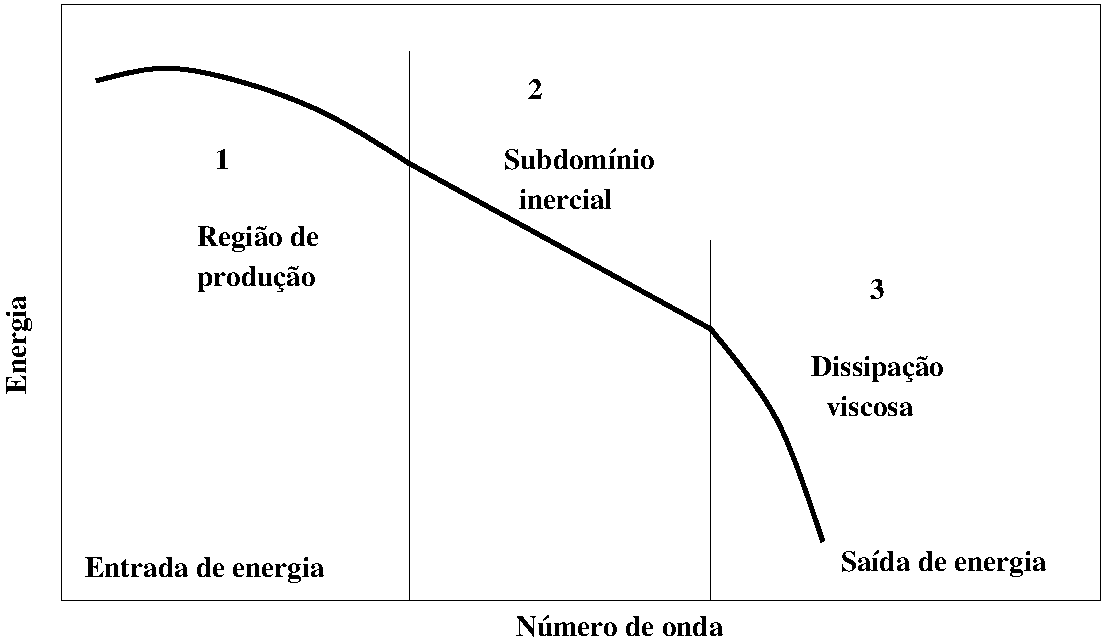
\includegraphics{Figuras/espectroesboco4.pdf}}
%\caption{Representação esquemática do espectro da ECT em escala $\log$-$\log$.}
%\FONTE{Adaptada de \citeonline{garratt/92}}
%\label{espectroesboco}
%\end{figure}
%
% \begin{figure}[!ht]
% \begin{center}
% \resizebox{13cm}{!}{\input{Figuras/espectroesboco5.pdftex_t}}
% \caption{Representação esquemática do espectro da ECT em escala $\log$-$\log$.}
% \FONTE{Adaptada de Garrat~\cite{garratt/92}}
% \label{espectroesboco}
% \end{center}
% \end{figure}
%
%Segundo \citeonline{frisch/96}, no SI o espectro de potência das principais grandezas turbulentas (velocidade, temperatura, umidade, etc) é caracterizado por uma lei de potência com inclinação $-5/3$, ou seja
%
%\begin{equation}
%S_{u}(k)=a k^{-5/3}
%\label{eqespectroturb}
%\end{equation}
%onde $a$ é uma constante de proporçao e $k$ é \textit{o número de onda}. Analogamente, a lei de potência com inclinação $-5/3$ é também obtida para $S_{u}(w)$, onde $w$ é a freqüência.
%
%\subsubsection{Estruturas coerentes em turbulência}
%
%As estruturas coerentes têm sido um assunto de grande relevância na pesquisa em turbulência~\cite{oliver/02}. Este interesse foi intensificado a partir de estudos que demonstraram que a presença dessas estruturas pode ser responsável por até $75\%$ dos fluxos turbulentos na camada da superfície atmosférica\footnote{A porção mais inferior da atmosfera, com extensão de aproximadamente $1$ a $2$ Km, é denominada camada limite atmosférica. Esta é a região mais influenciada diretamente por trocas de momento, calor e vapor de água na superfície da Terra.}~\cite{gao/89}, ou segundo outros autores por, em média, $40\%$ de todo o calor turbulento e fluxos de momento \cite{lu/94,oliver/02}.
%
%Não há uma definição precisa do que sejam estruturas coerentes. Segundo \citeonline{robinson/91} estruturas coerentes de grande escala constituem uma região do fluido turbulento que possui \textit{vorticidade}\footnote{O campo de vorticidade dado por $\omega (x,t)=\bigtriangledown \times u(x,t)$ é uma importante quantidade na caracterização e compreensão do fluxo turbulento. De forma geral, ele mede a rotação de um fluxo. Na turbulência 3-D, a vorticidade desempenha uma função quantitativa na qual a taxa média de energia dissipada $\varepsilon$ está relacionada com o quadrado da vorticidade pela relação $\varepsilon=-u\langle|\omega|^2\rangle$~\cite{ecke/05}.}\textit{coerente} sobre uma significativa extensão espacial. Essas estruturas podem ainda ser caracterizadas por uma região tridimensional, onde pelo menos uma das variáveis fundamentais do escoamento (componente de velocidade, massa específica, temperatura, etc.) apresenta significativa correlação com ela mesma ou com outra variável, num intervalo de espaço e/ou tempo suficientemente maior que as menores escalas locais do escoamento.
%
%As estruturas coerentes são características da turbulência de grande escala na camada da superfície atmosférica. Sob condições convectivas instáveis, elas são reconhecidas em séries temporais de flutuações de temperatura com uma gradual elevação da temperatura, seguida por uma súbita queda. Sob condições estáveis, este padrão se inverte e uma gradual queda é seguida por uma súbita elevação~\cite{oliver/02}. Nestas duas condições, a estrutura coerente é do tipo ``rampa''. 
%
%O efeito das condições de estabilidade sobre o comportamento em rampa das estruturas coerentes é uma conseqüência direta da distribuição espacial de fontes de calor e umidade. Por exemplo, durante o dia o ar aquecido está localizado próximo à superfície, assim a súbita queda de temperatura é devido à presença do ar mais frio que se desloca para baixo e, durante a noite, a súbita elevação da temperatura está associada com o ar mais quente que se desloca para baixo. Desde que a fonte de umidade esteja situada apenas na superfície, as estruturas coerentes presentes em séries temporais de flutuações de umidade mostram um padrão independente de estabilidade.
%
%\subsubsection{Intermitência em turbulência}
%
%A intermitência é um fenômeno relacionado à presença de raros, porém fortes gradientes de velocidade com acentuada localização no espaço ou no tempo. Esses gradientes são gerados por estruturas altamente coerentes (quase sempre não estacionárias) e são responsáveis pelo forte aumento da taxa de dissipação local da ECT~\cite{camussi/97}.
%
%Segundo \citeonline{frisch/96} uma função aleatória é intermitente se o quarto momento estatístico normalizado, a saber, a curtose definida como
%\begin{equation}
%K(r)=\frac{\langle u_{r}^4\rangle}{{\langle u_{r}^2\rangle}^2}
%\label{eqintermitencia}
%\end{equation}
%cresce sem limites quando $r\rightarrow 0$. Desta forma, pode-se afirmar que a curtose é uma grandeza estatística que quantifica a presença de fenômenos intermitentes em um escoamento turbulento, sendo um parâmetro que mede o grau de achatamento de uma \textit{Função de Distribuição de Probabilidade} (FDP). 
%
%A presença da intermitência em um sinal turbulento confere uma forma especial à sua FDP. Para o caso da turbulência atmosférica, as FDP's são, em geral, aproximadamente gaussianas nas maiores escalas do escoamento (com valores de curtose próximos de $3$) e fortemente não gaussianas em suas menores escalas, devido ao fenômeno da intermitência. As curvas da Figura~\ref{figpdfintermitente} são histogramas de $\Delta u_{r}=u(x+\Delta r)-u(x)$ obtidos para distâncias de separação (usando a hipótese de Taylor $\Delta r=U\Delta t$) dadas por $\Delta r=4,40,400$ e $4000$. Para dados amostrados a $60$ Hz essas distâncias correspondem a $\Delta t$ de $0.06,0.66,6.66,66.66$ segundos, respectivamente. Nas menores escalas de separação, ocorrem grandes flutuações com uma freqüência muito maior que aquela prevista para um processo gaussiano. Este fenômeno, diretamente ligado à intermitência do escoamento turbulento, aparece nas FDP's sob a forma de ``asas'' ou ``caudas'' prolongadas.
%Fernando
%
%\begin{figure}[ht]
%\centering \resizebox{13cm}{!}{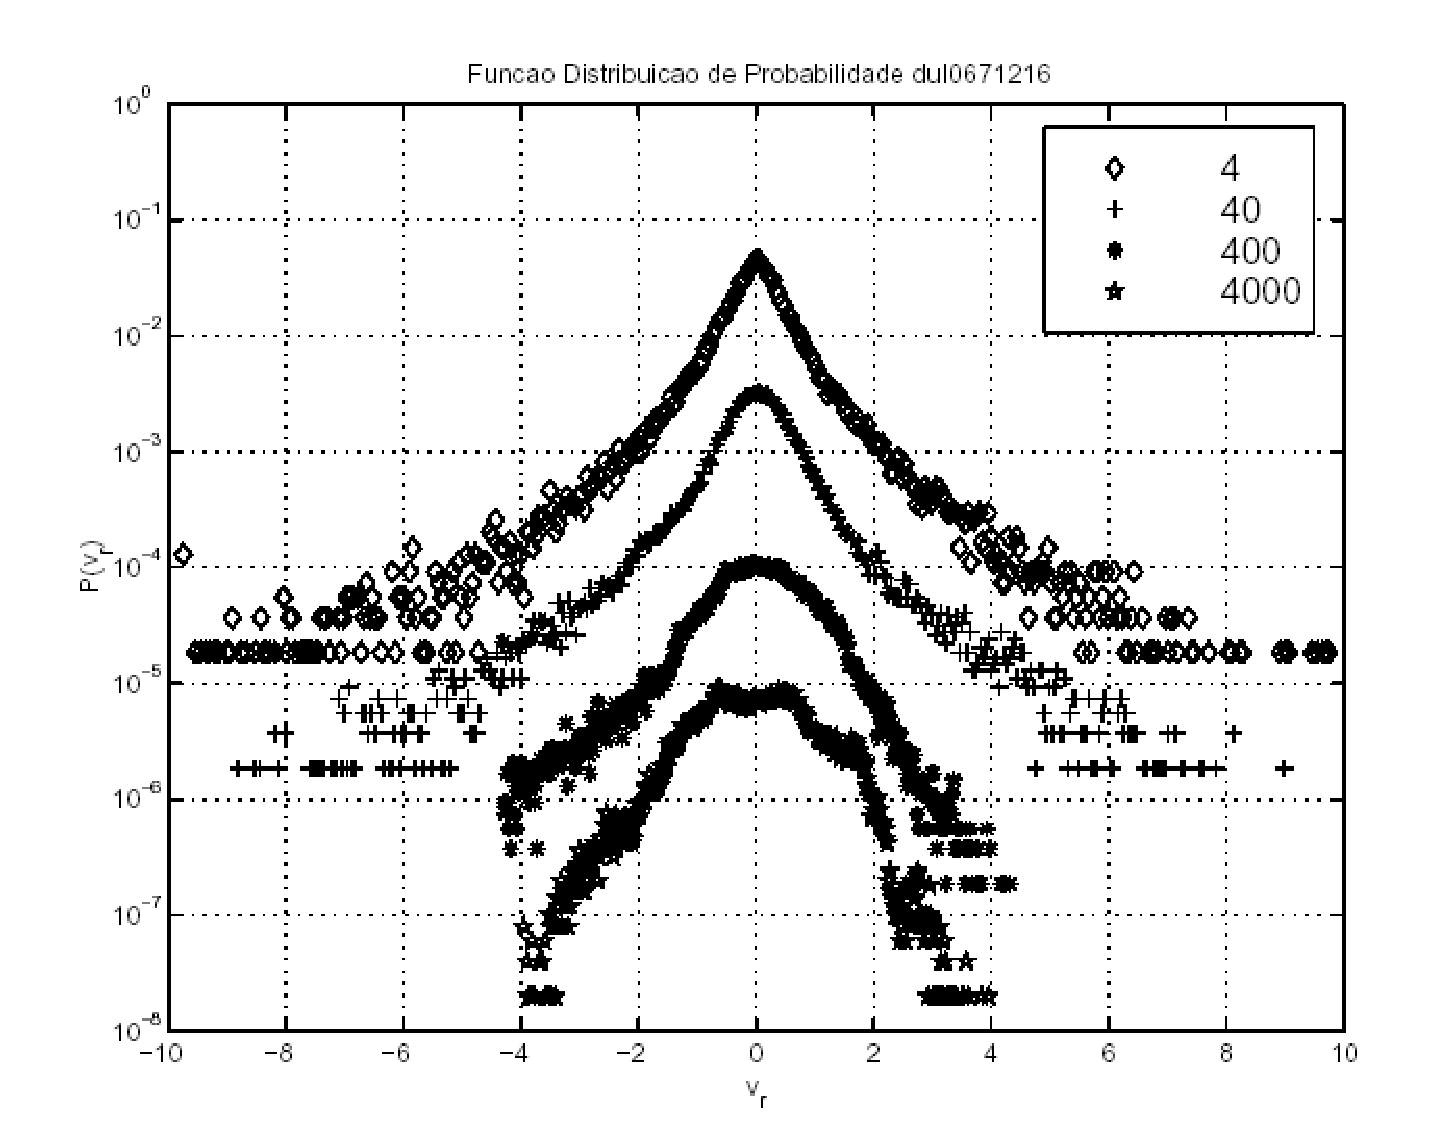
\includegraphics{Figuras/bolzan.pdf}}
%\caption{PDF's das diferenças de velocidade longitudinal dentro da copa da Floresta Amazônica, para valores de $\Delta r=4,40,400$ e $4000$.}
%\FONTE{\citeonline{bolzan/00}}
%\label{figpdfintermitente}
%\end{figure}
%
%\section{Caos e Turbulência}
%\label{seccaosurb}
%
%O desenvolvimento da teoria de sistemas dinâmicos caóticos, tem fornecido importantes subsídios à compreensão do fenômeno da turbulência. Uma conjectura feita por Landau foi a primeira tentativa para a descrição do surgimento da turbulência. Conforme sua teoria, o comportamento turbulento é causado por uma seqüência infinita de bifurcações de Hopf. Desta forma, cada vez que uma bifurcação ocorre, freqüências fundamentais\footnote{A cada nova freqüência associa-se um novo grau de liberdade ao sistema} são adicionadas ao sistema e a medida que cada vez mais freqüências ocorrem, o movimento torna-se cada vez mais turbulento~\cite{grebogi/83}. 
%
%A idéia defendida por Landau, de que um fenômeno complexo tal como a turbulência necessite de uma descrição complexa com infinitos graus de liberdade, foi contestada a partir do estudo de Lorenz que mostrou que um sistema com apenas três EDO's pode levar a comportamentos complexos e caóticos~\cite{argyris/94}. A concepção de Landau foi ainda fortemente questionada for \citeonline{ruelle/91}, sobretudo pela ausência tanto da sensibilidade às variações nas condições iniciais quanto de espectros contínuos em sua conjectura.
%
%O trabalho pioneiro de \citeonline{ruelltak/71} introduziu uma nova e promissora perspectiva para a compreensão do fenômeno turbulento. Esses autores foram os primeiros estudiosos a propor um possível mecanismo de transição de um fluxo laminar para um fluxo turbulento com base na teoria de sistemas dinâmicos, mais especificamente por meio de atratores caóticos. Com base nessa abordagem Ruelle, Takens, Feigenbaum, e outros autores, investigaram ``rotas para a turbulência'', ou seja, cenários (sucessões de bifurcações) nos quais um sistema com uma evolução temporal simples torna-se turbulento quando um ou mais de seus parâmetros são alterados~\cite{ruellelecture/90}.  
%
%\subsection{Bifurcação e rotas para a turbulência}
%
%
%O \textit{cenário Ruelle-Takens}~\cite{ruelltak/71} propõe uma rota baseada em três bifurcações consecutivas: ponto fixo $\longrightarrow$ ciclo limite $\longrightarrow$ toro\footnote{O toro $k$-dimensional $T^{k}$ pode ser entendido como o produto de $k$ círculos} $T^{3}$ $\longrightarrow$ atrator caótico (turbulência). Em outras palavras, movimentos quasiperiódicos sobre um toro $T^{3}$ (ou seja, com três freqüências incomensuráveis) podem perder estabilidade e surgir diretamente a turbulência~\cite{zeng/93,newhouse/78}. Esta rota é genérica e ocorre em diversos modelos matemáticos e em experimentos de laboratório, porém ela é uma rota de difícil compreensão teórica que as demais rotas mencionadas abaixo~\cite{zeng/93}.
%
%\citeonline{eckmann/81} propôs outra rota para a turbulência, que é conhecida como rota para a turbulência de Feigenbaum ou de duplicação de período: uma cascata de bifurcações de duplicações de período $p = 2^{n}(n=0,1,2,\ldots)$ que converge rapidamente para uma órbita aperiódica quando $n\rightarrow \infty$. Este cenário tem sido validado com grande êxito em diversas simulações numéricas e sistemas físicos. A duplicação de período tem sido observada em experimentos como a convecção de Rayleigh-Bénard~\cite{zeng/93}.
%
%A quarta rota, chamada de rota para a turbulência de Pomeau-Manneville, é através da intermitência~\cite{pomeau/80}. No contexto de sistemas caóticos, o termo \textit{intermitente} refere-se a alterações aleatórias entre um comportamento caótico e regular no tempo sem envolver nenhum grau de liberdade espacial. Este conceito é diferente do significado original da \textit{intermitência} na teoria hidrodinâmica da turbulência, que indica ``estouros'' aleatórios do movimento turbulento sobre a base de um fluxo laminar~\cite{zeng/93}. Nesta rota não há uma clara compreensão de quando o regime turbulento é alcançado nem da exata natureza desta turbulência~\cite{eckmann/81}. 
%
% Especificamente, pode-se afirmar que a rota Ruelle-Takens está relacionada a bifurcações do tipo Hopf, onde um par de autovalores complexos cruza o círculo unitário; a rota de Feigenbaum está associada com bifurcações do tipo Pitchfork, onde um autovalor cruza o círculo unitário em $-1$; e a rota Pomeau-Manneville está associada com bifurcações do tipo Sela-Nó, onde um autovalor cruza o círculo unitário em $1$. 
%
%
%A Tabela~\ref{tabbifurca} apresenta a evolução da dinâmica de um sistema, de um estado estacionário à um estado turbulento, sob a influência de diferentes sucessões de bifurcações.
%
%\begin{sidewaystable}
%\caption{Rotas para a turbulência com base em seqüências de bifurcações}
%\vspace{0.5cm}
%\begin{center}
%\resizebox{!}{3.6cm}{
%\begin{tabular}{c c c c c c c c c c c c}
%\hline 
%\multicolumn{1}{c}{\textbf{}} & \multicolumn{11}{c}{\textbf{}} \\
%\multicolumn{1}{c}{\textbf{Rotas}} & \multicolumn{11}{c}{\textbf{Seqüências de bifurcações}}\\
%\multicolumn{1}{c}{\textbf{}} & \multicolumn{11}{c}{\textbf{}}\\
%\cline{1-12}
%\hline 
%\textbf{} & Ponto & $\longrightarrow$ & Órbita & $\longrightarrow$ & Órbita & $\longrightarrow$ & Órbita & $\longrightarrow$ & $\cdots$ & $\longrightarrow$ & Movimento \\
%\textbf{Landau} & estacionário & (Hopf) & periódica & (Hopf) & periódica & (Hopf) & periódica & & (Hopf) & & turbulento \\
%\textbf{} & & & única &  & dupla &  & tripla & & & &  \\
%& & &  &  &  &  &  & & & &  \\
%\hline
%\textbf{Ruelle-} & Ponto & $\longrightarrow$ & Órbita & $\longrightarrow$ & Órbita & $\longrightarrow$ & Atrator &  &  & & \\
%\textbf{Takens} & estacionário & (Hopf) & periódica & (Hopf) & periódica & (Hopf) & caótico &  &  & &  \\
%\textbf{} & &  & única &  & tripla &  &  &  &  & & \\
%& & &  &  &  &  &  & & & &  \\
%\hline
%\textbf{} & Ponto & $\longrightarrow$ & Órbita & $\longrightarrow$ & Órbita & $\longrightarrow$ & Órbita & $\longrightarrow$ & $\cdots$ & $\longrightarrow$ & Atrator \\
%\textbf{Feigenbaum} & estacionário & (Hopf) & periódica & (Duplicação & periódica & (Duplicação & periódica &  & (Duplicação &  & Caótico \\
%\textbf{} & & & única & de & única & de & única &  & de &  &  \\
%\textbf{} & & & (período $T$) & período) & (período $2T$) & período) & (período $4T$) &  & período) &  &  \\
%& & &  &  &  &  &  & & & &  \\
%\hline
%\textbf{Pomeau-} & Ponto & $\longrightarrow$ & Órbita & $\longrightarrow$ & Movimento &  &  &  &  &  & \\
%\textbf{Manneville} & estacionário &(Hopf) & periódica &  & caótico &  &  &  &  &  &  \\
%\textbf{} & & & única &  & intermitente &  &  &  &  &  &  \\
%\hline
%\end{tabular}}
%\begin{flushleft}
%\tamfonte: {Adaptada de \cite{miles/84}}
%\end{flushleft}
%\label{tabbifurca}
%\end{center}
%\begin{flushleft}
%\vspace{0.2cm}\hspace{1.6cm}\tamfonte: {Adaptada de \citeonline{miles/84}}
%\end{flushleft}
%\end{sidewaystable}
%
%
%De modo geral, todas as rotas descritas acima, estão relacionadas à turbulência em seu estágio inicial (turbulência fraca), ou seja, quando a mesma pode ainda ser descrita por um número reduzido de graus de liberdade~\cite{chenmin/05}. Segundo \citeonline{zeng/93}, a compreensão do fenômeno turbulento será alcançada quando o mecanismo inicial que lhe deu origem for completamente entendido. Tal idéia justifica, em grande parte, a importância do estudo das rotas para a turbulência. Sob essa perspectiva, a turbulência fraca e caos possuem características em comum, já que ambos apresentam comportamentos irregulares em sua evolução temporal e podem ainda ser descritos por um conjunto reduzido de equações diferenciais determinísticas. Em contrapartida, a turbulência totalmente desenvolvida (com elevados números de Reynolds) envolve irregularidades de caráter temporal e espacial e só pode ser descrita por um número de graus de liberdade elevado.
%
%\subsection{Caracterização da turbulência via atratores caóticos}
%
%Desde que Lorenz introduziu seu modelo inspirado em dinâmica dos fluidos (conforme Seção~\ref{seccaos} deste capítulo), conjectura-se que a atmosfera possui um intrínseco limite de previsibilidade e que a dinâmica atmosférica é governada por um atrator caótico~\cite{weber/95}. 
%
%Diversos trabalhos confirmam a existência de atratores na atmosfera, com base em séries temporais turbulentas. Esses atratores foram detectados, de maneira geral, a partir da técnica da reconstrução de espaço de fase~\cite{tak/81}, que será discutida em detalhes no Capítulo~\ref{caputiltecnicas}. \citeonline{xin/01} detectaram a existência de atratores caóticos, com dimensão de correlação entre $3$ e $7$, a partir de dados turbulentos observados na camada limite atmosférica. Esses dados foram amostrados a $16$ Hz e incluem medidas de temperatura, umidade e velocidade do vento em três direções, obtidos na província de Gansu e em Beijing, China. 
%
% Diversos trabalhos confirmam a existência de atratores de baixa dimensão na atmosfera, com base em séries temporais turbulentas. Esses atratores foram detectados a partir da técnicas como a reconstrução de espaço de fase \ref{eqtakensreconst}, pelo algoritmo de Grassberger e Procaccia \ref{eqcorr1} e ainda pelo algoritmo de Wolf~\cite{wolf/85}. Xin \textit{et al} \cite{xin/01} detectaram a existência de atratores estranhos, com dimensão entre $3$ e $7$, a partir de dados turbulentos observados na camada limite atmosférica. Esses dados foram amostrados a $16$ Hz e incluem medidas de temperatura, umidade e velocidade do vento em três direções, obtidos na província de Gansu e em Beijing, China. 
%
%\citeonline{jaramillo/93} analisaram $24$ séries temporais de velocidade do vento e flutuações de temperatura, amostrados a $10$ Hz, em períodos de $30$ minutos, sobre condições atmosféricas instáveis, e concluiram que atratores caóticos com baixa dimensão, com dimensão de correlação entre $4$ e $6$, governam a dinâmica da baixa atmosfera de Ontário, Canadá. 
%
%A partir de dados de três componentes do vento, medidos em Almaraz (Cáceres, Espanha) à $18$ Hz, \citeonline{gallego/01} identificaram atratores caóticos para a turbulência convectiva com dimensão de correlação de aproximadamente $6$ e para a turbulência mecânica com dimensões de correlação variando entre $7$ e $9$. 
%
%Alguns trabalhos negam a existência de atratores caóticos na atmosfera. Nenhum indício de um atrator foi encontrado nas análises realizadas por \citeonline{weber/95} com base em séries temporais turbulentas das componentes vertical e horizontal da velocidade do vento, amostradas à $21$ Hz. \citeonline{loratrat/91} afirma que não há razão alguma para acreditar que um sistema dinâmico complexo, como o clima, possua um atrator de baixa dimensão associado. Segundo Lorenz, o valor da dimensão de correlação obtido em diversas análises, com base em séries temporais climáticas, pode estar relacionado à dimensão de um conjunto de subsistemas de baixa dimensão ``fracamente'' acoplados~\cite{loratrat/91}, e não à dimensão de um atrator associado ao sistema como um todo. A validade ou não deste cenário será investigada no Capítulo~\ref{caputiltecnicas}. Essa questão acerca da dimensão de um eventual atrator caótico associado à dinâmica da atmosfera está ainda em aberto, aguardando novos experimentos e o desenvolvimento de métodos inovadores de análise de séries temporais.
